\section{Power Supply}
This section will explain in detail the design of the power supply that was created to drive the various parts of the brick sorter. Three rails will be created, two using linear voltage regulators and one using a switching regulator. The power supply will be tested to verify that it conforms with the given performance requirements.
\subsection{Parts and Requirements}
The power supply described in this section is to have three voltage rails:
\begin{itemize}
	\item LEDs: 12v/1000mA.
	\item SERVO: 6v/1500mA.
	\item FPGA: 5v/1A, $\pm$\% max output voltage, min 80\% efficient.
\end{itemize}
The power supply itself is supplied with 15v. A list of components\footnote{Datasheets for all active components can be found in appendix \ref{app:datasheet}} was provided in order to facilitate the design process. These are the main components of the power supply:
\begin{itemize}
	\item LM2574: Step-Down Switching Regulator.
	\item NCP7812TG: 12v Linear Voltage Regulator.
	\item L7806cv: 6v Linear Voltage Regulator. 
\end{itemize}
Additionally, a PCB must be designed for the power supply.
\subsection{Design}
Since most of the components of the power supply are given, the task of design is mostly one of laying out the PCB. This is done by using Eagle\footnote{CadSoft EAGLE v7.4.0 Light Edition}. The schematics of the three different voltage rails can be seen in figure \ref{fig:psuschematic}.
The capacitors $C_3$ and $C_5$ are dimensioned according to the application circuit from their respective datasheet. They are omittable at low current operation or if the regulator is an appreciable distance from its power source. With no way of interpreting "appreciable distance" and operation being 1A and 1.5A for the 12v rail and the 6v rail respectively, it was decided to include them. Likewise, capacitors $C_4$ and $C_6$ serve to improve the transient response of the component.
The output and input of the linear voltage regulators is connected using a flyback diode. This is especially important on the 6V rail. This rail will be connected to the servomotor which, in a sense, is a coil, which can produce significant back electromotive force that could potentially damage the circuit.
\begin{figure}[h!]
	\begin{subfigure}{.48\linewidth}
		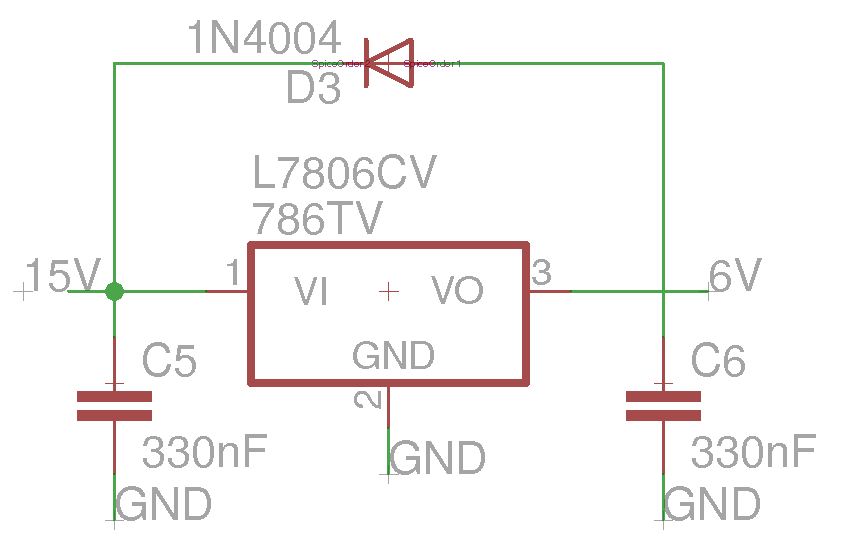
\includegraphics[width=\linewidth]{images/linear6v}
		\caption{Circuit for 6v rail.}
		\label{fig:psu6v}
	\end{subfigure}
	\begin{subfigure}{.48\linewidth}
		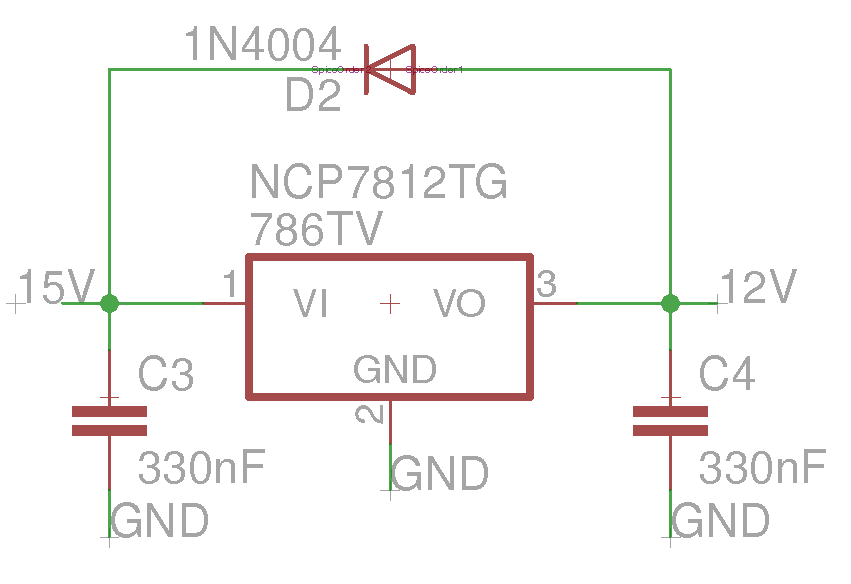
\includegraphics[width=\linewidth]{images/linear12v}
		\caption{Circuit for 12v rail.}
		\label{fig:psu12v}
	\end{subfigure}\\
	\begin{subfigure}{\linewidth}
		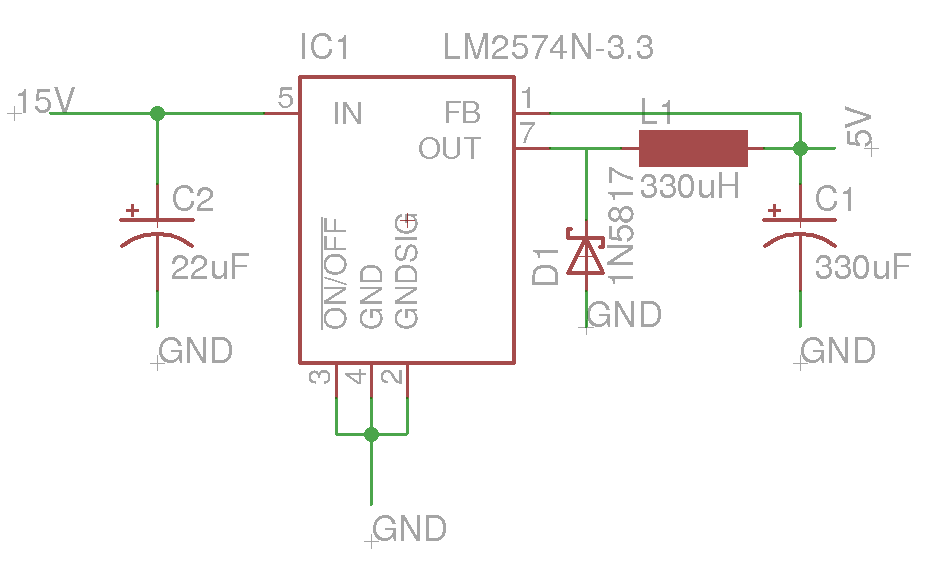
\includegraphics[width=\linewidth]{images/switch5v}
		\caption{Circuit for 5v rail.}
		\label{fig:psu5v}
	\end{subfigure}
	\caption{Schematics of the power supply.}
	\label{fig:psuschematic}
\end{figure}
The switching regulator in figure \ref{fig:psu5v} is designed as the typical applications design in the datasheet of the LM2574 \cite{lm2574}. This design is accompanied with a graph for dimensioning the size of the output inductance, $L_1$, see figure \ref{fig:inductorselect}. Since the IC will be supplied with 15V and a maximum load of 0.5A is required, the inductor necessary is 330$\mu$H. The value of the output capacitor, $C_1$ is determined according to 
\begin{eqnarray}
	C_\text{out}\geq&13300\frac{V_\text{in}(\text{MAX})}{V_\text{out}\cdot L(\mu\text{H})}(\mu\text{F})\\
	C_\text{out}\geq&13300\frac{15}{5\cdot 330} = 120.9(\mu\text{F})
\end{eqnarray} 
For this design, a 330$\mu$F capacitor is provided, which, while large, does fulfil the specification.
\begin{figure}
	\centering
	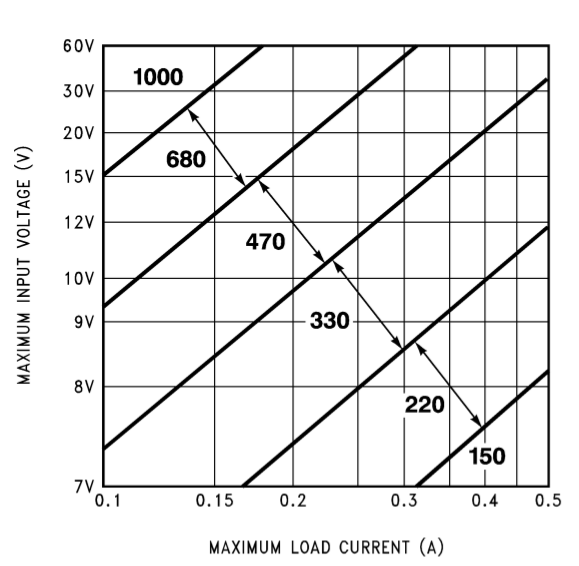
\includegraphics[width=.6\linewidth]{images/inductorselector}
	\caption{Graph showing the necessary inductance at various voltages and loads.}
	\label{fig:inductorselect}
\end{figure}